\documentclass[tikz,crop]{standalone}

\usepackage[T1]{fontenc}
\usepackage[tt=false,type1=true]{libertine}
\usepackage[varqu]{zi4}
\usepackage{newtxmath}
\usepackage[dvipsnames]{xcolor}
\usepackage{tikz,listings}
\usepackage{bbding}
\usetikzlibrary{arrows,fit,positioning,shadows,shapes,shapes.arrows}
\definecolor{palet1}{HTML}{c7522a}
\definecolor{palet2}{HTML}{e5c185}
\definecolor{palet3}{HTML}{fbf2c4}
\definecolor{palet4}{HTML}{74a892}
\definecolor{palet5}{HTML}{008585}
\colorlet{ctop}{palet1}
\colorlet{cleft}{palet2}
\colorlet{cmid}{palet4}
\colorlet{cright}{palet3}

\begin{document}
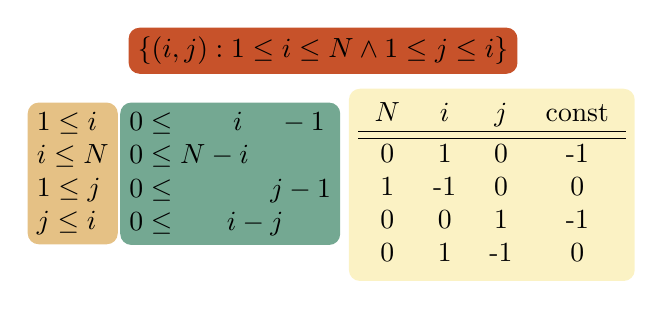
\begin{tikzpicture}
  \path
  (2em,0) node[rounded corners, fill=ctop, anchor=south west] {$\{ (i,j) : 1 \le i \le N \land 1 \le j \le i\}$}
  (0,-1em) node[rounded corners, fill=cleft, anchor=north , align=left] {
    $1 \le i$ \\
    $i \le N$ \\
    $1 \le j$ \\
    $j \le i$
  }
  (2,-1em) node[rounded corners, fill=cmid, anchor=north, align=left] {
    $0 \le \phantom{N}\quad i\phantom{+j}-1$ \\
    $0 \le N-i\phantom{+j}$ \\
    $0 \le \phantom{N +i+}j-1$ \\
    $0 \le \phantom{N +}i-j$}
  (3.5,-0.5em) node[rounded corners, fill=cright, anchor=north west] {
    \begin{tabular}{cccc}
      $N$ & $i$ & $j$ & const\\
      \hline
      \hline
      0   & 1   & 0   & -1   \\
      1   & -1  & 0   & 0    \\
      0   & 0   & 1   & -1   \\
      0   & 1   & -1  & 0
    \end{tabular}
  }
  ;
\end{tikzpicture}
\end{document}
